% Questo file definisce lo stile che verrà applicato
% ad ogni pagina di contenuto
\documentclass[a4paper,11pt]{article}

\usepackage{ifthen}
\usepackage[
 a4paper,
 top=2.5cm,
 bottom=2.5cm,
 left=1.5cm,
 right=1.5cm,
 head=30pt
]{geometry}
\usepackage[italian]{babel}
\usepackage[utf8x]{inputenc}
\usepackage[T1]{fontenc}
\usepackage{fancyhdr}
\usepackage[colorlinks=true, urlcolor=black, citecolor=black, linkcolor=black]{hyperref}
\usepackage{tabularx}
\usepackage{multirow}
\usepackage{booktabs}
\usepackage{color}
\usepackage[dvipsnames]{xcolor}
\usepackage{graphicx}
\usepackage{eurosym}
\usepackage{amsmath}
\usepackage{relsize}
\usepackage{placeins}
\usepackage{ltablex}
\usepackage{float}

\usepackage[multidot]{grffile}
\usepackage{xcolor,colortbl}
\definecolor{lightblue}{HTML}{56B4E6}
\definecolor{blue}{HTML}{2953A1}
\definecolor{darkblue}{HTML}{1E396E}
\usepackage{longtable}

\usepackage[toc,page]{appendix}
\renewcommand\appendixtocname{Appendice}
\renewcommand{\appendixpagename}{Appendice}

\newcommand\pagenumberingnoreset[1]{\gdef\thepage{\csname @#1\endcsname\c@page}}

% Cambia il font 
\renewcommand*\rmdefault{qhv}

% ***STILE PAGINA***
\pagestyle{fancy}
\fancyhf{}
\setlength{\headheight}{1cm} 
% No indentazione paragrafo
\setlength{\parindent}{0pt}

% ***INTESTAZIONE***
\newcommand\textline[4][t]{%
  \noindent\parbox[#1]{.333\textwidth}{\raisebox{-0.40\height}{#2}}%
  \parbox[#1]{.333\textwidth}{\centering #3}%
  \parbox[#1]{.333\textwidth}{\raggedleft #4}%
}

\lhead{
	\textline[t]{
\includegraphics[width=1cm, keepaspectratio=true]{../../../Template/Logo/Logo.png}}{\progettoShort}{\documento}
}

\renewcommand{\headrulewidth}{0.4pt}  %Linea sotto l'intestazione

% ***PIÈ DI PAGINA***
\lfoot{\textit{\gruppoLink}\\ \footnotesize{\email}}
\rfoot{\thepage} %per le prime pagine: mostra solo il numero romano
\cfoot{}
\renewcommand{\footrulewidth}{0.4pt}   %Linea sopra il piè di pagina


% Ridefinisce command \paragraph{} andando a capo ogni dopo la parola dentro le parentesi ed ha la possibiltà di enumerazione fino a n cifre modificando il numero dentro "secnumdepth"
\usepackage{titlesec}

\setcounter{secnumdepth}{7}
\setcounter{tocdepth}{7}


% Visualizza paragraph come una section
\titleformat{\paragraph}{\normalfont\normalsize\bfseries}{\theparagraph}{1em}{}
\titlespacing*{\paragraph}{0pt}{3.25ex plus 1ex minus .2ex}{1.5ex plus .2ex}

\titleformat{\subparagraph}{\normalfont\normalsize\bfseries}{\thesubparagraph}{1em}{}
\titlespacing*{\subparagraph}{0pt}{3.25ex plus 1ex minus .2ex}{1.5ex plus .2ex}

\makeatletter
\newcounter{subsubparagraph}[subparagraph]
\renewcommand\thesubsubparagraph{%
  \thesubparagraph.\@arabic\c@subsubparagraph}
\newcommand\subsubparagraph{%
  \@startsection{subsubparagraph}    % counter
    {6}                              % level
    {\parindent}                     % indent
    {3.25ex \@plus 1ex \@minus .2ex} % beforeskip
    {0.75em}                           % afterskip
    {\normalfont\normalsize\bfseries}}
\newcommand\l@subsubparagraph{\@dottedtocline{6}{13em}{5.5em}} %gestione dell'indice
\newcommand{\subsubparagraphmark}[1]{}
\makeatother

\makeatletter
\newcounter{subsubsubparagraph}[subsubparagraph]
\renewcommand\thesubsubsubparagraph{%
  \thesubsubparagraph.\@arabic\c@subsubsubparagraph}
\newcommand\subsubsubparagraph{%
  \@startsection{subsubsubparagraph}    % counter
    {7}                              % level
    {\parindent}                     % indent
    {3.25ex \@plus 1ex \@minus .2ex} % beforeskip
    {0.75em}                           % afterskip
    {\normalfont\normalsize\bfseries}}
\newcommand\l@subsubsubparagraph{\@dottedtocline{7}{16em}{6.5em}} %gestione dell'indice
\newcommand{\subsubsubparagraphmark}[1]{}
\makeatother

%Generali
\newcommand{\capitolato}{C5 - Monolith: An interactive bubble provider}
\newcommand{\progettoShort}{Monolith}
\newcommand{\progetto}{Monolith: An interactive bubble provider}
\newcommand{\gruppo}{NPE Developers}
\newcommand{\gruppoLink}{\href{https://gitlab.com/npe-developers}{NpeDevelopers}}
\newcommand{\email}{\href{mailto:npe.developers@gmail.com}{\textcolor{blue}{npe.developers@gmail.com}}}
\newcommand{\password}{NP3Devel0pers}
\newcommand{\myincludegraphics}[2][]{%
	\setbox0=\hbox{\phantom{X}}%
	\vtop{
		\hbox{\phantom{X}}
		\vskip-\ht0
		\hbox{\includegraphics[#1]{#2}}}
}




%Componenti del gruppo
\newcommand{\RM}{Riccardo Montagnin}
\newcommand{\MT}{Manuel Turetta}
\newcommand{\FB}{Francesco Bazzerla}
\newcommand{\SL}{Stefano Lia}
\newcommand{\LD}{Luca Dario}
\newcommand{\DC}{Diego Cavestro}
\newcommand{\ND}{Nicolò Dovico}

%Ruoli
\newcommand{\Pm}{Project Manager}
\newcommand{\Am}{Amministratore}
\newcommand{\AmP}{Amministratori}
\newcommand{\An}{Analista}
\newcommand{\AnP}{Analisti}
\newcommand{\Dev}{Sviluppatore}
\newcommand{\DevP}{Sviluppatori}
\newcommand{\Ver}{Verificatore}
\newcommand{\VerP}{Verificatori}
\newcommand{\Progr}{Programmatore}
\newcommand{\ProgrP}{Programmatori}
\newcommand{\Prog}{Progettista}
\newcommand{\ProgP}{Progettisti}



%Firme
\newcommand{\RMFirma}{\myincludegraphics[scale = 0.5]{../../../Template/Firme/RM.png}}
\newcommand{\MTFirma}{\myincludegraphics[scale = 0.5]{../../../Template/Firme/MT.png}}
\newcommand{\FBFirma}{\myincludegraphics[scale = 0.5]{../../../Template/Firme/FB.png}}
\newcommand{\SLFirma}{\myincludegraphics[scale = 0.5]{../../../Template/Firme/SL.png}}
\newcommand{\LDFirma}{\myincludegraphics[scale = 0.5]{../../../Template/Firme/LD.png}}
\newcommand{\DCFirma}{\myincludegraphics[scale = 0.5]{../../../Template/Firme/DC.png}}
\newcommand{\NDFirma}{\myincludegraphics[scale = 0.5]{../../../Template/Firme/ND.png}}

%Professori e proponente
\newcommand{\TV}{Prof. Tullio Vardanega}
\newcommand{\RC}{Prof. Riccardo Cardin}
\newcommand{\RB}{Red Babel}
\newcommand{\proponente}{Red Babel}

%Documenti
\newcommand{\Gl}{Glossario}
\newcommand{\glossario}{\textit{\Gl\_v.2.0.0.pdf}}
\newcommand{\AdR}{Analisi dei Requisiti}
\newcommand{\analisiDeiRequisiti}{\textit{\AdR\_v.2.0.0.pdf}}
\newcommand{\AdRvDue}{AnalisiDeiRequisiti}
\newcommand{\NdP}{Norme di Progetto}
\newcommand{\normeDiProgetto}{\textit{\NdP\_v.2.0.0.pdf}}
\newcommand{\PdP}{Piano di Progetto}
\newcommand{\pianoDiProgetto}{\textit{\PdP\_v.2.0.0.pdf}}
\newcommand{\SdF}{Studio di Fattibilità}
\newcommand{\studioDiFattibilita}{\textit{\SdF\_v.2.0.0.pdf}}
\newcommand{\PdQ}{Piano di Qualifica}
\newcommand{\pianoDiQualifica}{\textit{\PdQ\_v.2.0.0.pdf}}
\newcommand{\VI}{Verbale Interno}
\newcommand{\VE}{Verbale Esterno}
\newcommand{\ST}{Specifica Tecnica}
\newcommand{\MU}{Manuale Utente}
\newcommand{\DDP}{Definizione di Prodotto}

%Periodo di progetto
\newcommand{\ARM}{Analisi dei Requisiti di Massima}
\newcommand{\ARD}{Analisi dei Requisiti in Dettaglio}
\newcommand{\PA}{Progettazione Architetturale}
\newcommand{\PD}{Progettazione di Dettaglio}
\newcommand{\COD}{Codifica}
\newcommand{\VV}{Verifica e Testing Finale}

%Consegne
\newcommand{\RR}{Revisione dei Requisiti}
\newcommand{\RP}{Revisione di Progettazione}
\newcommand{\RQ}{Revisione di Qualifica}
\newcommand{\RA}{Revisione di Accettazione}


%Formattazione
\newcommand{\termine}[1]{\textit{#1}\small{$_G$}}
\newcommand{\link}[1]{\href{#1}{\textcolor{blue}{\texttt{#1}}}} 

% Testi ricorrenti
\newcommand{\scopoProdotto}{L'obiettivo di questo progetto è la realizzazione di un \termine{SDK} che permetta la creazione di bolle interattive, le quali, successivamente, verranno utilizzate all'interno dell'applicazione di messaggistica istantanea open source \termine{Rocket.chat}. \\
Dopo la realizzazione di tale \termine{SDK}, è proposto lo sviluppo di un'applicazione in grado di sfruttare l'\termine{SDK} per implementare un uso originale. L'applicazione scelta dal \termine{team} consiste nella bolla lista-spesa e nei suoi vari utilizzi all'interno della piattaforma \termine{Rocket.chat}.
}
\newcommand{\descrizioneGlossario}{Al fine di mantenere questo documento compatto e di facile lettura è stato realizzato un glossario esterno contenente tutte le definizioni dei termini che più comunemente verranno presentati al lettore.  
Tale glossario si ritrova all'interno del file \glossario, e contiene tutti e soli i termini che vengono marcati con una \textit{G} a pedice.
}
\newcommand{\riferimentiNormativi}{
	\begin{itemize}
		\item \textbf{Norme di Progetto}: \normeDiProgetto
		\item \textbf{\termine{Capitolato} d'appalto C5: Monolith - An Interactive bubble provider} \\
			  \link{http://www.math.unipd.it/~tullio/IS-1/2016/Progetto/C5.pdf}
	\end{itemize}
}

% Comandi per generare l'intro
\newcommand{\documento}{\NdP}
\newcommand{\versione}{2.0.3}
\newcommand{\redatori}{\FB\\ & \LD\\ & \ND\\ &\DC}
\newcommand{\revisori}{\LD}
\newcommand{\approvazione}{\DC}
\newcommand{\statoapprovazione}{Non approvato}
% Quando il documento sarà approvato, inserire all'interno del comando seguente la data nel formato GG mese AAAA dove GG è il giorno a due cifre, mese è il mese scritto per esteso con la prima lettera minuscola, e AAAA è l'anno a quattro cifre
\newcommand{\dataApprovazione}{** 2017}
\newcommand{\uso}{Interno}
\newcommand{\destinatari}{\gruppo \\ & \TV\\ & \RC\\}

\newcommand{\sommario}{Il presente documento descrive le regole e le procedure cui i membri del gruppo \gruppo\ sono tenuti ad essere conformi nello sviluppo del progetto \progetto{}. \\ L'organizzazione più naturale dei contenuti di questo documento è per processi (quelli adottati e adattati a partire dallo standard ISO/IEC 12207).
}

\newcommand{\modifiche}{
3.0.0 & Approvazione del documento - Creare nuova versione del documento & \SL & \Pm & 07/05/2017 \\\midrule
2.1.0 & Verifica documento - Correzione errori & \LD & \Ver & 04/05/2017 \\\midrule
2.0.4 & Aggiunta la nota riguardante la forma del \MU\ di \progettoShort\ - In seguito a quanto deciso in data 03 maggio 2017 e riportato nell'apposito verbale & \ND & \Am & 04/05/2017 \\\midrule
	2.0.3 & Modificata la sezione delle metriche per la codifica - Aggiungere regole più precise per facilitare la stesura del codice & \ND & \Am & 28/03/2017 \\\midrule
2.0.2 & Aggiunte sezioni mancanti - Migliorare la profondità del documento come segnalato nella correzione in seguito alla \RP & \SL & \Am & 27/03/2017 \\
\midrule
2.0.1 & Riorganizzata la sezione degli strumenti - Aggiungere chiarezza su quale strumento sia usato per quale attività & \SL & \Am & 26/03/2017 \\
\midrule
2.0.0 & Approvazione del documento - Creare nuova versione del documento & \DC & \Pm & 04/03/2017 \\
\midrule 
1.1.0 & Verifica del documento - Correzioni errori & \LD & \Ver & 04/03/2017 \\
\midrule 
	1.0.2 & Aggiunta metriche - Aggiunta profondità come segnalato nella correzione in seguito alla \RR & \ND & \Am & 28/02/2017 \\
	\midrule
	1.0.1 & Aggiornamenti sezioni 3 e 4 - Aggiunta ampiezza come segnalato nella correzione in seguito alla \RR & \ND & \Am & 27/02/2017 \\
	\midrule
	1.0.0 & Approvazione - Creare la prima versione del documento & \SL & \Pm & 04/01/2016 \\
	\midrule
	0.4.0 & Verifica sottosezione 4.4 - Correzione errori & \RM & \Ver & 29/12/2016 \\\midrule
	0.3.1 & Stesura sottosezione 4.4 - Aggiunte norme sul processo di formazione & \DC & \Ver & 29/12/2016 \\\midrule
	0.3.0 & Verifica sezione 4 - Correzione errori & \RM &\Ver & 27/12/2016 \\\midrule
	0.2.0 & Verifica sezione 3 - Correzione errori & \RM & \Ver & 24/12/2016 \\\midrule
	0.1.0  & Verifica sezioni 1 e 2 - Correzioni errori & \RM & \Ver & 23/12/2016\\\midrule
    0.0.5 & Stesura sezione 4 - stabilire norme per il coordinamento e pianificazione & \DC & \Am & 21/12/2016 \\\midrule
    0.0.4 & Stesura sezione 2 - Definizione dei processi primari per il progetto & \LD & \Am & 20/12/2017 \\\midrule
    0.0.3 & Stesura sezione 1 e modifica del template - Introduzione al documento & \FB & \Am & 18/12/2016 \\\midrule
    0.0.2 & Stesura sezione 3 - Definizione dei processi di supporto  & \ND & \Am & 17/12/2016 \\\midrule
    0.0.1 & Creazione del template - Inizio documento & \SL & \Am & 15/12/2016 \\\midrule
}


\usepackage{listings}
%\lstset{ %
%commentstyle=\color{ForestGreen}
%}

\begin{document}

% Questo file contiene il layout della prima pagina
\pagenumbering{gobble}

\title{
\includegraphics[width=8cm, keepaspectratio=true]{../../../Template/Logo/Logo.png} \\
	\documento \\
	Versione \versione
}
\date{\dataApprovazione}

\maketitle

\begin{center}

\begin{tabular}{ r | l }
  \textbf{Ruolo} & \textbf{Componente} \\
  Redazione & \redatori \\
  Revisione & \revisori \\
  Approvazione & \approvazione \\
  \\
  Stato & \statoapprovazione \\
  Uso & \uso \\
  Destinatari & \destinatari
\end{tabular}
\end{center}

\begin{center}
\textbf{Sommario\\}
\sommario \\
\vspace{1.5cm}\email
\end{center}

\clearpage

\pagenumbering{arabic}
%Questo file si occupa di generare la tabella delle modifiche
\pagenumbering{Roman}

\begin{center}
    \Large{\textbf{Registro delle modifiche}}
    	\\\vspace{0.5cm}
    	\normalsize
    \begin{tabularx}{\textwidth}{cXXcc}
        \textbf{Versione} & \textbf{Modifica - Motivazione} & \textbf{Autore} & \textbf{Ruolo} & \textbf{Data} \\\toprule
        \modifiche
    \end{tabularx}
\end{center}

\newpage



\tableofcontents

\newpage

\pagenumbering{arabic}



\section{Introduzione}
\subsection{Scopo del documento}
Questo documento vuole definire le strategie che il \termine{team} ha deciso di adottare per perseguire gli obiettivi di qualità di processo e di prodotto ricercati. A tal fine è necessaria una costante attività di verifica e validazione del lavoro svolto in modo da poter rilevare e correggere le anomalie che potrebbero nascere.

\subsection{Scopo del prodotto}
\scopoProdotto

\subsection{Glossario}
\descrizioneGlossario

\subsection{Riferimenti}
\subsubsection{Normativi}
\riferimentiNormativi

\subsubsection{Informativi}
\begin{itemize}
	\item \textbf{\AdR}: \analisiDeiRequisiti;
	\item \textbf{\PdP}: \pianoDiProgetto;
	\item \textbf{\textit{Slide} dell'insegnamento di Ingegneria del Software}: \\
		  \link{http://www.math.unipd.it/~tullio/IS-1/2016/}
	\item \textbf{\textit{Standard} ISO/IEC 9126}: Product quality \\
	 	  \link{https://en.wikipedia.org/wiki/ISO/IEC\_9126}
	\item \textbf{\textit{Standard} tecnici ISO/IEC 15504}: Software process assessment \\
		  \link{https://en.wikipedia.org/wiki/ISO/IEC\_15504}
	\item \textbf{Ciclo di Deming (\termine{PDCA})}: Miglioramento dei processi \\
		  \link{https://en.wikipedia.org/wiki/PDCA}
\end{itemize}

\newpage
\section{Processi primari}
\subsection{Processo di fornitura}
In questa sezione verrà spiegato il processo di fornitura da parte del gruppo \gruppo.

\subsubsection{Studio di Fattibilità}
Alla pubblicazione dei capitolati d'appalto il \textit{\Pm} avrà il compito fissare un
numero sufficiente di riunioni volte alla discussione e al confronto tra i membri del \termine{team}.
In seguito, gli \textit{\AnP} dovranno stilare lo \textit{\SdF} in base a quanto
emerso nelle riunioni. Tale documento sarà articolato nei seguenti punti:
\begin{itemize}
	\item \textbf{Descrizione:} descrizione generale di ciò che viene richiesto
	dal capitolato.
	\item \textbf{Dominio Applicativo:} descrizione dell'ambito di utilizzo del
	prodotto richiesto e delle caratteristiche che deve avere il prodotto finale.
	\item \textbf{Dominio Tecnologico:} descrizione delle tecnologie impiegate
	nello sviluppo del progetto richiesto.
	\item \textbf{Potenziali Criticità:} elenco delle possibili problematiche che potrebbero
	sorgere durante lo sviluppo del prodotto richiesto, individuando quindi punti
	critici ed eventuali rischi.
	\item \textbf{Analisi di mercato} descrizione delle potenzialità del dominio applicativo.
	\item \textbf{Valutazione Finale:} piccolo elenco dei lati positivi e negativi del capitolato scelto.
\end{itemize}

\subsubsection{Pianificazione}
Per garantire una buona probabilità di successo del capitolato è stato redatto il documento \PdP\ contente la pianificazione dei periodi, la scelta del modello di vita del software e le \termine{milestones} per la consegna. \\
Infine per garantire qualità ai processi e al prodotto è stato redatto il documento \PdQ.

\paragraph{Strumenti}

\subparagraph{GanttChart}
Lo strumento per la costruzione dei diagrammi di Gantt contenuti nel \PdP\ che abbiamo scelto è \termine{GanttChart}.
Le ragioni che ci hanno portato a questa scelta sono:

\begin{itemize}
\item Facilità di utilizzo.
\item Problematiche legate all'estrapolazione del \termine{diagramma di Gantt} da \termine{Wrike}.
\end{itemize}

\subsubsection{Esecuzione e Controllo}
E' compito dei membri del gruppo eseguire i processi descritti in questo documento e monitorare continuamente il loro stato. Questa attività è necessaria anche per l'individuazione, registrazione, analisi e risoluzione dei problemi che potrebbero verificarsi.

\subsubsection{Revisione e Valutazione}
Questa attività è destinata ai \Ver\ che hanno il compito di attuare le attività di verificazione e validazione rispettivamente per i processi e per il prodotto. Una volta ottenuti i risultati, tramite essi, si deve valutare lo stato dei processi. Nel caso qualcuno di essi non superi la verifica, il gruppo \gruppo\ dovrà discutere su come intervenire per migliorare quel processo.

\subsection{Processo di sviluppo}
\subsubsection{Analisi dei Requisiti}
Ultimato lo \textit{\SdF} gli \textit{\AnP} dovranno stilare l'\textit{\AdR} che dovrà 	essere strutturata nel seguente modo.
\paragraph{Classificazione dei requisiti}
Dovrà essere stilato un elenco di requisiti, emersi durante le riunioni interne
e/o esterne. Questo compito spetta agli \textit{\AnP}. I requisiti dovranno
essere classificati secondo la seguente codifica:

\begin{center}
R-[Importanza][Tipo][Identificativo]
\end{center}
\begin{itemize}
	\item \textbf{Importanza:} può assumere questi valori:
  		\begin{itemize}
    		\item \textbf{1:} indica un requisito obbligatorio.
    		\item \textbf{2:} indica un requisito desiderabile.
    		\item \textbf{3:} indica un requisito facoltativo.
  		\end{itemize}
  	\item \textbf{Tipo:} può assumere questi valori:
  		\begin{itemize}
   		 	\item \textbf{F:} indica un requisito funzionale.
    		\item \textbf{Q:} indica un requisito di qualità.
    		\item \textbf{P:} indica un requisito prestazionale.
    		\item \textbf{V:} indica un requisito di vincolo.
  		\end{itemize}
  	\item \textbf{Identificativo:} indica il codice identificativo del requisito, è univoco e deve essere indicato in forma gerarchica.
\end{itemize}
Per ogni requisito si dovranno inoltre indicare:
\begin{itemize}
  \item \textbf{Descrizione:} una breve descrizione del requisito, che chiarisca tutti i punti di esso senza lasciare spazio a possibili ambiguità.
  \item \textbf{Fonte:} la fonte può essere una delle seguenti:
  \begin{itemize}
    \item \textit{\termine{Capitolato}}: deriva direttamente dal testo del capitolato.
    \item \textit{Verbale}: deriva da un incontro verbalizzato, seguito dall'identificativo dell'incontro.
    \item \textit{Interno}: deriva da discussioni interne al \termine{team}.
    \item \textit{Caso d'uso}: deriva da uno o più casi d'uso, seguito dall'identificativo del caso o dei casi d'uso.
  \end{itemize}
\end{itemize}

\paragraph{Classificazione dei casi d'uso}
Ogni requisito sarà specificato da un diagramma di caso d'uso e sarà rappresentato in questo modo:
\begin{center}
  UC[Identificativo]
\end{center}
dove:
\begin{itemize}
  \item\textbf{Identificativo}: è il codice gerarchico univoco, rappresentato in numeri, per identificare ogni caso d'uso.
\end{itemize}
Inoltre per ogni caso d'uso dovranno essere indicati:
\begin{itemize}
  \item\textbf{Titolo}: indica il titolo del caso d'uso.
  \item\textbf{Descrizione}: breve descrizione del caso d'uso.
  \item\textbf{Attori}: indica gli attori, sia principali che secondari, coinvolti nel caso d'uso.
  \item\textbf{Precondizione}: indica la condizione che deve essere verificata prima
  dell'esecuzione del caso d'uso.
   \item\textbf{Precondizione}: indica la condizione che deve essere verificata dopo dell'esecuzione del caso d'uso.
  \item\textbf{Scenario principale}: descrizione composta dal flusso dei casi d'uso
  figli.
  \item\textbf{Scenari alternativi}: descrizione composta dai casi d'uso che non
  appartengono al flusso principale di esecuzione.
  \item\textbf{Estensioni}: indica quali sono tutte le estensioni, se presenti.
  \item\textbf{Inclusioni}: indica quali sono tutte le inclusioni, se presenti.
  \item\textbf{Generalizzazioni}: indica quali sono tutte le generalizzazioni,
  se presenti.
  \item\textbf{Postcondizione}: indica la condizione che deve essere verificata dopo
  l'esecuzione del caso d'uso.
\end{itemize}

\paragraph{Obiettivi dell'analisi}

\begin{itemize}
\item Individuare tutti i requisiti tramite riunioni interne, tra i membri del gruppo, o esterne, con i committenti.
\item Ogni requisito deve essere concordato da tutti i membri.
\end{itemize}

\paragraph{Strumenti}

\subparagraph{Astah}
Lo strumento per la costruzione degli use cases che abbiamo scelto è \termine{Astah}.
Le ragioni che ci hanno portato a questa scelta sono:
\begin{itemize}
\item Disponibilità dello strumento di costruire \termine{Diagrammi dei casi d'uso}.
\item Possibilità di avere la licenza in modo gratuito essendo studenti.
\end{itemize}



\subsubsection{Progettazione}

\paragraph{Requisiti per i progettisti}
I \textit{\ProgP} sono responsabili delle attività di progettazione e sono tenuti ad avere:
\begin{itemize}
\item
Profonda conoscenza di tutto ciò che riguarda il processo di sviluppo del software.
\item
Capacità di saper anticipare i cambiamenti.
\item
Notevole inventiva per riuscire a trovare una soluzione progettuale accettabile anche in mancanza di una metodologia che sia sufficientemente espressiva.
\item
Capacità di individuare con rapidità e sicurezza le soluzioni più opportune.
\end{itemize}

L'attività di Progettazione coinvolge due attività, le quali:
\begin{itemize}
\item \textbf{Progettazione architetturale}
\item \textbf{Progettazione in dettaglio}
\end{itemize}

\paragraph{Progettazione architetturale}

\subparagraph{Descrizione}
L'attività di progettazione architetturale descrive le attività per realizzare la struttura dell'architettura ed è rivolta ai programmatori. Essi hanno il compito di trasformare i requisiti software delineati nel documento \AdR{} in un'architettura che descrive ad alto livello le componenti software. Inoltre è necessario assicurarsi che tutti i requisiti siano soddisfatti dalle componenti individuate, il tutto, poi, va appositamente documentato nella sezione dedicata del \DDP{}. \\
Per arrivare, dunque, ad una definizione soddisfacente dell'architettura dei prodotti software è necessario svolgere delle attività, che dovranno portare i seguenti risultati:

\begin{enumerate}
\item \textbf{Definizione delle componenti}: Individuazione delle componenti ad alto livello che andranno a costituire il sistema. Dovranno essere definite poi le interazioni tra le componenti, in modo da far capire il funzionamento del prodotto realizzato.
\item \textbf{Scelta delle tecnologie}: Dovranno essere individuate tutte le \termine{librerie} o \termine{framework} necessari per la realizzazione del prodotto. Ognuna dovrà essere descritta con annessa spiegazione del suo utilizzo.
\item \textbf{Definizione dei Design Pattern}: I \textit{Progettisti} devono inoltre individuare, se ritenuti necessari, eventuali \termine{Design Pattern} per la definizione dell'architettura di sistema. Per ognuno di essi si dovranno fornire le seguenti informazioni:
\begin{itemize}
\item descrizione testuale.
\item descrizione grafica, tramite un \termine{diagramma di sequenza} che ne spiega il funzionamento.
\item motivazione dell'utilizzo.
\item descrizione di come viene applicato il pattern al progetto.
\end{itemize}
\item  \textbf{Tracciamento delle componenti}: Ogni componente dovrà essere tracciata ed associata ad almeno un requisito. In tal modo sarà possibile essere certi che tutti i requisiti, individuati durante l'attività di analisi, siano soddisfatti e che non esistano componenti che non soddisfino requisiti. Il tracciamento potrà essere fatto tramite gli opportuni script in \termine{Python} e la scrittura dei file \termine{JSON}.
\item \textbf{Definizione Test d'integrazione}: definite le componenti, i \textit{Progettisti}, dovranno opportunamente definire dei test che possano verificare efficacemente le interazioni tra le componenti.
\item \textbf{Definizione Test di Sistema}: i \textit{Progettisti} dovranno progettare dei test di sistema in modo che tutti i requisiti siano verificati, al fine di garantire correttezza al programma.
\item \textbf{Definizione Tesi di validazione}: i \textit{Progettisti} devono infine progettare dei test di validazione che verranno poi provati in periodo di collaudo. Tali test dovranno coprire tutte le funzionalità del programma al fine di mostrarne il valore e correttezza.
\end{enumerate}


\subparagraph{Diagrammi UML}
La progettazione deve utilizzare le seguenti tipologie di diagrammi \termine{UML}:
\begin{itemize}
\item
\textbf{Diagrammi dei \textit{\termine{package}}}: illustrano i vari raggruppamenti di classi in una unità di livello più alto.
\end{itemize}

\subparagraph{Classificazione dei package}
I package vengono identificati univocamente da una descrizione nella forma:
\begin{center}
\textit{PackagePadre::Package\_nome}
\end{center}

Dove \textit{PackagePadre} sono tutti i package che stanno a livello superiore come cartella ed anch'essi sono definiti con la stessa norma tipografica. \\
\textit{Package\_nome} invece identifica il nome del package in se. Sarà compito dei \textit{Progettisti} trovare un nome esplicativo al fine di semplificare la comprensione delle sue funzionalità ai \textit{Programmatori}. Ogni package, infine, dovrà essere fornito di una descrizione che ne spieghi il funzionamento.

\subparagraph{Obiettivi della progettazione architetturale}
L'attività di progettazione si pone i seguenti obiettivi:
\begin{itemize}
\item Realizzare una struttura architetturale per l'applicativo  resistente alle modifiche, senza che l'intera struttura venga compromessa e/o nuovamente messa in discussione.
\item Progettare un software con le caratteristiche che sono state elencate e descritte nella fase di analisi dei requisiti.
\item Identificare i \termine{Design Patterns} più utili al fine di creare un'architettura coesa, con poco accoppiamento e con un'elevata riusabilità.
\item Individuare le interfacce necessarie all'interazione tra le componenti tra loro e con l'ambiente.
\item Perseguire una buona qualità per l'architettura.
\end{itemize}

\paragraph{Progettazione in dettaglio}

\subparagraph{Descrizione}
L'attività di Progettazione in dettaglio definisce le unità realizzative, ovvero i moduli che poi andranno a formare l'intero sistema. Tali moduli devono essere specificati in modo dettagliato e devono essere descritte le interazioni tra di essi.
Al fine di ottenere una buona progettazione in dettaglio dovranno essere svolte delle attività, che dovranno portare come risultato i seguenti risultati:

\begin{enumerate}
\item \textbf{Definizione delle classi}: tramite le tecniche di modularizzazione citate in precedenza devono essere individuate tutte le classi necessarie per la realizzazione del prodotto.
\item \textbf{Tracciamento delle classi}: ogni classe deve mirare a soddisfare uno o più requisiti. Ciò è fatto sia per garantire il soddisfacimento dei requisiti sia per evitare di ottenere classi che non soddisfano nulla.
\item \textbf{Spiegazione del funzionamento}: Ogni classe deve essere opportunamente spiegata nella sezione dedicata del documento \DDP{} in ogni sua parte e funzionalità.
\item \textbf{Definizione dei Test di Unità}: per verificare il corretto funzionamento di una classe, i \textit{Progettisti} devono pianificare dei test adatti a tale scopo. Essi verranno poi implementati dai \textit{Programmatori}, perciò è necessario mantenerne traccia.
\end{enumerate}

\subparagraph{Diagrammi UML}
La progettazione deve utilizzare le seguenti tipologie di diagrammi \termine{UML}:
\begin{itemize}
\item
\textbf{Diagrammi di classe}: illustrano una collezione di elementi dichiarativi di un modello come classi e tipi, assieme ai loro contenuti e alle loro relazioni.
\item
\textbf{Diagrammi di attività (opzionali)}: illustrano il flusso di operazioni relativo ad un'attività e utilizzati soprattutto per descrivere la logica di un algoritmo.
\item
\textbf{Diagrammi di sequenza}: descrivono una determinata sequenza di azioni dove tutte le scelte sono già state effettuate. In tali diagrammi non compaiono pertanto scelte né flussi alternativi. Verranno descritti solo per le operazioni reputate interessanti, cioè con un alto tassi di utilizzo e con una adeguata complessità, in modo che risultino interessanti da descrivere.
\end{itemize}

\subparagraph{Tecniche di modularizzazione}

I \textit{Progettisti} prima di iniziare l'attività di progettazione in dettaglio, devono necessariamente adottare delle tecniche di modularizzazione al fine di garantire una progettazione di qualità. Queste tecniche devono, infatti, garantire una scomposizione efficace delle componenti individuate nell'attività di progettazione architetturale. \\
Queste tecniche devono essere incentrate sul riuso del codice, in modo da garantire una sviluppo più rapido del prodotto. A tal fine saranno stabilite successivamente delle metriche per garantire che ciò avvenga correttamente.

\subparagraph{Classificazione delle classi}

Le classi vengono univocamente identificate dalla seguente forma di scrittura:
\begin{center}
\textit{NomePackage::NomeClasse}
\end{center}

Dove \textit{NomePackage} è il nome della componente ad alto livello che contiene la classe. Essa viene scritta nella forma precedentemente citata. \\
Mentre \textit{NomeClasse} è il nome del modulo attribuito dai \textit{Progettisti}.

\subparagraph{Obiettivi della progettazione in dettaglio}
La fase di progettazione si pone i seguenti obiettivi:
\begin{itemize}
\item Soddisfare i requisiti obbligatori fissati dal committente.
\item Avere una chiara idea delle parti(classi,metodi e e variabili) che si andranno successivamente a codificare nel periodo che va dal \RP\ alla \RQ
\item Descrivere in maniera appopriata e comprensibile a uno sviluppatore esterno i metodi,le variabili e le classi codificate. Come successivamente descritto.
\item Descrivere in dettaglio le interazioni tra le varie componenti utilizzando i \textit{Design Patterns} scelti durante l'attività di progettazione architetturale.
\item Seguendo quanto detto per la progettazione architetturale, anche quella in dettaglio deve perseguire gli obbiettivi di coesione, basso accoppiamento e riusabilità dei moduli.
\end{itemize}

\paragraph{Strumenti}

\subparagraph{Astah}
Lo strumento per la costruzione dell'architettura di sistema e dettaglio che abbiamo scelto è \termine{Astah}.
Le ragioni che ci hanno portato a questa scelta sono:
\begin{itemize}
\item Disponibilità dello strumento di costruire \termine{Diagrammi dei package} per la progettazione architetturale.
\item Disponibilità dello strumento di costruire \termine{Diagrammi delle classi}, \termine{Diagrammi di sequenza} e \termine{Diagrammi delle attività} per la progettazione in dettaglio.
\end{itemize}

\subsubsection{Codifica}
\paragraph{Descrizione}
La fase di codifica ha come obiettivo quello di passare, nel miglior modo possibile, dalla soluzione architetturale realizzata dai \textit{\ProgP} a quella finale eseguibile da un calcolatore.
In questa fase i responsabili della codifica sono i \textit{\ProgrP} e questi sono tenuti a seguire le seguenti \termine{best practice}, con lo scopo di produrre il prodotto designato nella fase di progettazione.

\paragraph{Formattazione}
Per semplificare il compito del \textit{\Progr} è fondamentale delineare uno standard di formattazione.
Esso coincide nei seguenti punti:

\begin{itemize}
\item Mantenere l'indentazione standard di \termine{IntelliJ IDEA} composta da quattro(4) spazi.

\item Inserire le parentesi di apertura in modo \termine{inline}.

\item Utilizzare spazi vuoti nel codice sorgente in modo da suddividere il file in paragrafi migliorandone lettura e comprensione.

\item Inserire sempre le parentesi di apertura e di chiusura di una istruzione condizionale anche quando è presente solo uno \termine{statement} all'interno del suo corpo. In tal modo verrà facilitata la comprensione e manutenzione del codice.

\item Suddividere logicamente il codice in diversi file.

\item Cercare di incapsulare più possibile il codice e non di creare funzioni e/o classi con una eccessiva quantità di codice.
\end{itemize}

\paragraph{Commenti}
All'interno del codice è fondamentale inserire una buona quantità di commenti al fine di facilitare la comprensione, sia ad un lettore esterno, sia allo stesso programmatore a distanza di tempo.
Di seguito sono suggeriti alcuni metodi di inserimento di commenti che saranno utilizzati dal gruppo:

\begin{itemize}
\item Cercare di inserire commenti di facile comprensione a tutti.

\item Commentare tutto ciò che non è immediato nel codice.

\item Evitare l'inserimento di commenti alla fine di una riga di codice ma preferire tale inserimento nella riga sovrastante ad essa.

\item Commentare sempre tutte le istruzioni condizionali se considerate non di facile comprensione.

\item Tenere sempre aggiornati i commenti relativi all'eventuale codice che si va a modificare, al fine di evitare problemi di inconsistenza con esso.

\item Evitare commenti superflui o umoristici in quanto in caso di \termine{commit} resteranno nella storia dello sviluppo del software.
\end{itemize}

\paragraph{Nomi}
Lo schema di denominazione è uno dei supporti più determinanti per la comprensione del codice.
Di seguito sono elencate le tecniche per raggiungere un buon utilizzo dei nomi.

\begin{itemize}
\item Seguire la pratica \termine{camel case} per la denominazione delle variabili locali.
\item Seguire la pratica \termine{PascalCase} per la denominazione delle classi.
\item Seguire la pratica UPPER\textunderscore CASE per la denominazioni delle variabili statiche costanti.
\item Utilizzare uno nome significativo per le variabili, le classi ed i metodi scritti, al fine di rendere superflua qualunque documentazione.
\item Evitare di utilizzare gli stessi nomi per elementi diversi.
\item Utilizzare nome composti da una sola lettera solamente per le variabili che identificano un indice all'interno di una istruzione ciclica.
\item Cercare di utilizzare nomi diverse per tutte le classi, anche se facenti parte di packages diversi.
\item Per le variabile private delle classi si usa la pratica \termine{camel case} precedute da un underscore 
\end{itemize}

\paragraph{Rami di sviluppo}

La \termine{Repository} su \termine{GitHub} sarà divisa in due branch, in entrambi i progetti che si andranno a realizzare (\termine{SDK} e applicativo):
\begin{enumerate}
\item \textbf{master}: costituirà il ramo contenente le versioni stabili del codice.
\item \textbf{development}: ramo che può contenere codice non testato o in fase di sviluppo.
\end{enumerate}


Tutti i \textit{Programmatori} dovranno sviluppare nel ramo \textit{development}. Potranno, una volta terminata e testata la parte assegnata, effettuare una richiesta per il \termine{merge} sul \textit{master}.

\subparagraph{Effettuare una pull request}

Una volta che il codice è stato completamente scritto, documentato e testato, il \Prog{} dovrà, oltre ad avvisare gli altri membri del gruppo con gli appositi strumenti, richiedere una \termine{pull-request}, tramite GitHub, sul ramo-master. Il \Pm{}, a quel punto, deve decidere se accettare o meno la richiesta dopo una breve discussione con i \VerP{}, che a loro volta devono aver controllato e testato il codice.

\paragraph{Gestione dei problemi}

Quando vengono individuati dei malfunzionamenti o dei problemi che non si riescono a risolvere da soli, si dovrà, tramite lo strumento GitHub, aprire una \textit{issue}. Essa consiste nel descrivere un problema al quale successivamente l'intero \termine{team} si impegnerà a risolvere. Lo scopo principale di quest'attività è quello, non solo di trovare una soluzione accettabile, ma anche quello di coinvolgere utenti esterni al gruppo, in modo da poter creare, e successivamente sfruttare, una \termine{community} di persone. Inoltre, ciò è fatto anche per quegli utenti, che usando l'\textit{Monolith} o \textit{Bring-it} da poco, si trovano innanzi a problemi già affrontati, in modo tale da aiutarli a trovare presto la soluzione ideale.

\paragraph{Analisi statica}

Per effettuare l’analisi statica del codice scritto è possibile utilizzare \termine{SonarQube}. Questo strumento ad ogni \termine{push} effettuata nel \termine{Repository} controllerà i parametri di qualità statici definiti dalle metriche trovate dal gruppo. Nel caso in cui, tali parametri, non fossero superati i \textit{Programmatori} dovranno provvedere, al più presto, a correggere gli errori con un successivo \termine{push}. Ciò è necessario poiché non sarà possibile fare il \termine{merge} delle modifiche dal ramo \textit{development} al ramo \textit{master} senza che i parametri di qualità vengano superati.
  
\paragraph{Ricorsione}
La ricorsione va evitata il più possibile. Per ogni funzione ricorsiva sarà necessario valutare il costo in termini di occupazione della memoria e bisognerà associare ad esso una prova di correttezza.
Valutare la memoria occupata dalla funzione sarà obbligatorio in quanto le funzioni ricorsive possono facilmente non terminare occupando tutto lo stack della memoria andando quindi in \termine{stack overflow}.

\paragraph{Obiettivi della codifica}
La fase di codifica si pone i seguenti obiettivi:
\begin{itemize}
\item Realizzare la demo come progettata nel \DDP.
\item Trasformare in un linguaggio adatto tutte le funzioni e le classi con i loro relativi attributi 
\end{itemize}

\paragraph{Strumenti}

\subparagraph{IntelliJ IDEA}
L'ambiente di sviluppo integrato (\termine{IDE}) scelto per lo sviluppo e la manutenzione del progetto è \termine{IntelliJ IDEA}. Le ragioni che hanno portato a questa scelta sono le seguenti:
\begin{itemize}
\item Disponibilità di svariati \termine{plugin} per lo sviluppo, in particolare per \termine{Meteor.js}.
\item Buona conoscenza di questo strumento d parte di tutti i componenti del \termine{team} maturata durante il corso di laurea.
\item Possesso di una completa integrazione con i metodi di versionamento \termine{Git}.
\item Abilità di autocompletamento del codice \termine{JavaScript} scritto.
\item Possesso di un \termine{debugger} \termine{JavaScript}.
\end{itemize}

\subsubsection{Integrazione}
In questo periodo si cerca di integrare le varie parti del nostro applicativo e del nostro sdk in maniera che funzioni correttamente interfacciandosi in  correttamente tra di loro. Per fare questo abbiamo sviluppato degli appositi test che andremo successivamente ad elencare.
Questa attività deve essere svolta in maniera ottimale e precisa dai \textit{progettisti}, che dovranno avere una chiara idea del funzionamento delle parti che hanno sviluppato e una idea abbastanza precisa del funzionamento delle parti che gli altri .\textit{progettisti} hanno sviluppato. Una volta finita l'integrazione tra le varie componenti si procederà a verificare tramite dei test appositi il completo e corretto funzionamento di tutto l'applicativo e l'SDK

\paragraph{Requisiti per i progettisti}
I \textit{\ProgP} sono responsabili delle attività di integrazione e sono tenuti ad avere:
\begin{itemize}
\item
Profonda conoscenza di tutto quello che hanno sviluppato.
\item
Capacità di saper effettuare piccoli cambiamneti al loro codice per integrarlo al meglio nel ecosistema del intero progetto.
\item
Conoscere le parti sviluppate da altri per poterle integrare al meglio.
\item
Avere competenze necessarie per sviluppare le parti mancanti di software che permettono l'interazione tra le varie parti.
\item
Capacità di individuare con rapidità i bug e i requisiti non soddisfatti che l'applicativo finale comporta.
\end{itemize}

\paragraph{Obiettivi per l'integrazione}
Il periodo in cui si svolge l'integrazione pone i seguenti obiettivi:
\begin{itemize}
\item Avere un applicativo che unisce tutte le parti software sviluppate indipendentemente e non, dai vari progettisti.
\item Controllare, e nel caso correggere eventuali errori e bug apparsi durante l'integrazione
\end{itemize}

\subsubsection{Sistemi Operativi}
Ogni componente del team ha scelto di usare il proprio sistema operativo preferito. Sono, dunque, utilizzate attualmente tre diversi sistemi: MacOs,  ArchLinux e Windows 10. L'uso di sistemi diversi, però, non risulta essere un problema per il corretto funzionamento del software poiché la programmazione avviene principalmente lato server rendendo cosi ininfluente la scelta del sistema operativo del client.

\newpage 
\section{Processi di supporto}
\subsection{Processo di documentazione}
In questa sezione verranno descritti tutti i metodi ed i procedimenti utilizzati per registrare le informazioni prodotte dal ciclo di vita di un processo o di una attività.

\subsubsection{Descrizione}
Tratteremo di seguito tutte le convenzioni adottate dal \termine{team} per produrre i documenti dove registrare le informazioni sopra dette, e tutti i metodi per standardizzare la loro  stesura, verifica e approvazione. \\
I documenti vengono classificati come:
\begin{itemize}
  \item \textit{Interni} se il loro utilizzo rimane interno al \termine{team};
  \item \textit{Esterni}: se la loro distribuzione avviene anche alle componenti esterne al gruppo, come ad esempio il committente e/o il proponente.
\end{itemize}

I documenti \textit{approvati} dal \textit{\Pm} devono avere un nome strutturato nel seguente modo:
\begin{itemize}
  \item La prima lettera del documento deve essere maiuscola;
  \item Il nome non deve contenere spazi e deve essere scritto in \termine{camel case} per identificare; 
  \item La versione del documento deve essere indicata nella parte finale del nome in forma numerica
  \begin{center}
  \textit{NomeDelDocumento\_v.1.0.0}
  \end{center}\
\end{itemize}
Inoltre nel documento deve essere specificato il suo scopo (facilmente comprensibile dal suo titolo) e  nel diario delle modifiche dovranno essere elencati i soggetti che hanno preso parte alla stesura, modifica, verifica e approvazione del documento stesso.

\subsubsection{Strumenti}
Per la stesura dell'intera documentazione è stato scelto di utilizzare \textit{\termine{LaTeX}} in quanto questo \termine{linguaggio di markup} permette di avere uno
standard comune ed evitare possibili conflitti e incompatibilità derivanti
dall'utilizzo di software differente.

\subsubsection{Struttura del documento}
\paragraph{Prima pagina}
Ogni documento deve avere nella prima pagina le seguenti informazioni:
\begin{itemize}
  \item Nome del gruppo;
  \item Logo del progetto;
  \item Nome del progetto;
  \item Nome del documento;
  \item Versione del documento;
  \item Data di creazione del documento;
  \item Data di ultima modifica del documento;
  \item Stato del documento;
  \item Nome e cognome del redattore del documento;
  \item Nome e cognome del verificatore del documento;
  \item Nome e cognome del responsabile approvatore del documento;
  \item Uso del documento;
  %\item Lista di distribuzione del documento;
  \item Destinatari del documento;
  \item Un sommario contenente una breve descrizione del documento.
\end{itemize}

\paragraph{Diario delle modifiche}
La seconda pagina di ogni documento deve contenere il diario delle modifiche. In questa tabella vengono inserite tutte le modifiche effettuate dai vari redattori del documento. Ogni
riga della tabella deve contenere le seguenti informazioni:
\begin{itemize}
  \item \textbf{Descrizione}: descrizione della modifica apportata;
  \item \textbf{Autore e Ruolo}: autore della modifica e ruolo che esso ricopre;
  \item \textbf{Data}: data della modifica apportata;
  \item \textbf{Versione}: versione del documento dopo la modifica.
\end{itemize}

\paragraph{Indice}
In ogni documento, dopo il diario delle modifiche, deve essere presente un
indice di tutte le sezioni. In presenza di tabelle e/o immagini queste devono
essere indicate con i relativi codici identificati.

\paragraph{Formattazione generale delle pagine}
La formattazione della pagina, oltre al contenuto, prevede un'intestazione e un
piè di pagina. \\
L'intestazione della pagina contiene:
\begin{itemize}
  \item Nome del progetto;
  \item Nome del documento;
  \item Logo del gruppo.
\end{itemize}
Il piè di pagina contiene:
\begin{itemize}
  \item Il nome del gruppo;
  \item Email del gruppo;
  \item Numero della pagina corrente.
\end{itemize}

\subsubsection{Norme tipografiche}
Le seguenti norme tipografiche indicano i criteri riguardanti
l'ortografia e la tipografia di tutti i documenti.

\paragraph{Stili di testo}
\begin{itemize}
  \item \textbf{Grassetto}: Il grassetto deve essere utilizzato per evidenziare parole
  particolarmente importanti, negli elenchi puntati o nelle frasi;
  \item \textbf{Corsivo}: Il corsivo deve essere utilizzato nelle seguenti
  situazioni:
  \begin{itemize}
    \item Ruoli: ogni riferimento a ruoli di progetto va scritto in corsivo;
    \item Documenti: ogni riferimento a un documento va scritto in corsivo;
    \item Stati del documento: ogni stato del documento va scritto in corsivo;
    \item Citazioni: ogni citazione va scritta in corsivo;
    \item Glossario: ogni parola presente nel glossario, oltre ad avere un pedice, deve
    essere scritta in corsivo.
  \end{itemize}
\end{itemize}

\paragraph{Composizione del testo}
\begin{itemize}
   \item \textbf{Glossario}: il pedice \termine{} verrà utilizzato in corrispondenza di vocaboli presenti nel \textit{\glossario}.
\end{itemize}

\paragraph{Formati}
\begin{itemize}
   \item \textbf{Date}: le date presenti nei documenti devono seguire lo standard seguente:
   \begin{center}
     GG-MM-AA
   \end{center}
   dove:
   \begin{itemize}
   		\item GG rappresenta il giorno.
     	\item MM rappresenta il mese;
     	\item AA rappresenta l'anno;
   \end{itemize}
   \item \textbf{Ore}: le ore presenti nei documenti devono seguire lo standard seguente (a 24 ore):
   \begin{center}
     hh:mm
   \end{center}
   dove:
   \begin{itemize}
     \item hh: rappresentano le ore;
     \item mm: rappresentano i minuti.
   \end{itemize}
   \item \textbf{Nome del documento}: per riferirsi al nome del documento si
   dovrà utilizzare il comando \termine{LaTeX} \\ \verb|\Nome del documento| garantendo in questo modo la corretta sintassi;
   \item \textbf{Nome del gruppo}: per riferirsi al nome del gruppo si dovrà
   utilizzare il comando \termine{LaTeX} \verb|\gruppo| garantendo in questo modo la corretta sintassi;
   \item \textbf{Nome del progetto}: per riferirsi al nome del progetto si dovrà
   utilizzare il comando \termine{LaTeX} \verb|\progetto| garantendo in questo modo la corretta sintassi;
   \item \textbf{Link sito del gruppo}: per riferirsi al link del sito del gruppo si dovrà
   utilizzare il comando \termine{LaTeX} \verb|\gruppoLink| garantendo in questo modo la corretta sintassi;
   \item \textbf{Email del gruppo}: per riferirsi all'indirizzo email del gruppo si dovrà
   utilizzare il comando \termine{LaTeX} \verb|\email| garantendo in questo modo la corretta sintassi;
   \item \textbf{Nome del proponente}: per riferirsi al nome del proponente, ovvero \proponente, si dovrà
   utilizzare il comando \termine{LaTeX}  \verb|\proponente| garantendo in questo modo la corretta
   sintassi.
\end{itemize}

\subsubsection{Componenti grafiche}
\paragraph{Tabelle}
Tutte le tabelle presenti all'interno del documento devono avere una didascalia
ed un codice identificativo univoco.

\paragraph{Immagini}
Le immagini inserite nel documento devono essere in formato \termine{PNG}.

\subsubsection{Composizione email}
Di seguito vengono descritte le norme da applicare nella composizione delle email.

\paragraph{Destinatario}
\begin{itemize}
  \item Interno: l'indirizzo da utilizzare è \email;
  \item Esterno: l'indirizzo del destinatario varia a seconda si tratti del Prof. Tullio Vardanega \\ (\link{tullio.vardanega@math.unipd.it}), del Prof. Riccardo Cardin (\link{rcardin@math.unipd.it}) o i proponenti del progetto.
\end{itemize}

\paragraph{Mittente}
\begin{itemize}
  \item Interno: l'indirizzo è di colui che scrive la email;
  \item Esterno: l'indirizzo da utilizzare è \email e può usarlo unicamente il \Pm.
\end{itemize}

\paragraph{Oggetto}
L'oggetto della mail deve essere esplicito, comprensibile e conciso in modo da rendere
immediato il riconoscimento del contenuto.

\paragraph{Corpo}
Il testo del corpo della mail deve essere esaustivo. All'interno del
testo ci si potrà riferire a un ruolo preciso all'interno del team o a un destinatario univoco.

\paragraph{Allegati}
È sconsigliato l'invio di allegati tramite mail in quanto è preferibile infatti condividere file all'interno del gruppo tramite strumenti più adatti, come \termine{Google Drive}.

\subsubsection{Produzione di documenti}
I documenti prodotti come sopra detto verranno innanzitutto creati con il linguaggio di markup \termine{LaTeX}, e successivamente salvati in formato \termine{PDF}. I tipi di documento prodotti sono i seguenti.

\paragraph{\SdF}
Questo documento riporta le motivazioni che hanno portato l'intero
\termine{team} all'accettazione dello sviluppo del progetto scelto. E' un documento interno e la lista di distribuzione riguarda i committenti.

\paragraph{\NdP}
Questo documento riporta le convenzioni, strumenti e
norme che il \termine{team} ha scelto di adottare durante  lo sviluppo del progetto. Questo
documento è interno e la lista di distribuzione riguarda i committenti.

\paragraph{\PdP}
Questo documento descrive come il \termine{team} gestisce le risorse
temporali e umane a disposizione e come sono stati valutati e trattati i rischi. Questo documento è esterno e la lista di distribuzione comprende sia i committenti che i proponenti.

\paragraph{\PdQ}
Questo documento descrive in che maniera l'intero \termine{team} cerca di soddisfare gli obiettivi di qualità del progetto. Questo documento è esterno e la lista di distribuzione comprende sia i committenti che i proponenti.

\paragraph{\AdR}
Questo documento dà una visione di insieme dei casi d'uso del progetto e dei requisiti stabiliti da esso. Contiene inoltre i diagrammi delle attività di interazione tra utente e sistema sviluppato e i servizi che il progetto una volta concluso andrà ad erogare. È un documento esterno e la lista di distribuzione comprende committenti che i proponenti.

\paragraph{\ST}
L'intento del suddetto documento è dare una visione generale del prodotto e delle sue richieste. Più nello specifico verrà mostrata una progettazione ad alto livello, basata su diagrammi dei \termine{package} per la descrizione delle componenti, diagrammi di sequenza per descrivere gli scenari d'uso e diagrammi di attività. Verranno inoltre elencati i software che saranno utilizzati per la realizzazione del progetto. Questo è un documento esterno e la sua lista di distribuzione comprende  sia i committenti che i proponenti.

\paragraph{\DDP}
L'intento di tale documento è fornire una progettazione dettagliata del
prodotto. In esso verranno forniti tutti i dettagli implementativi del prodotto, fondamentali in fase di codifica, che comprenderanno diagrammi \termine{UML} delle classi e i relativi metodi. Questo è un documento esterno e la sua lista di distribuzione comprende  sia i committenti che i proponenti.

\paragraph{\glossario}
Questo documento viene prodotto al fine di dare una spiegazione dettagliata dei termini tecnici e degli acronimi acronimi utilizzati nell'intera documentazione. La sua lista di distribuzione comprende i committenti che i proponenti ed è quindi un documento esterno.

\paragraph{\MU}
Questo documento fornisce all'utente una guida delle funzionalità e dei servizi offerti dal prodotto. Essendo una guida destinata all'utente è un documento esterno e la sua lista di distribuzione comprende i sopracitati utenti.

\paragraph{Verbale}
Questo documento ha lo scopo di riassumere in modo formale le discussioni effettuate e le decisioni prese durante le riunioni. I verbali, come i documenti, sono classificati in:
\textbf{interni} ed \textbf{esterni}. In particolare i verbali esterni, essendo ufficiali, devono essere redatti dal \Pm. \\
Ogni verbale dovrà essere denominato nel seguente modo:
\begin{center}
  \textit{{Verbale}\_{Numero del verbale}\_{Tipo di verbale}\_{Data del verbale}}
\end{center}
dove:
\begin{itemize}
  \item \textbf{Numero del verbale} è numero identificativo univoco del verbale;
  \item \textbf{Tipo di verbale} identifica se si tratta di un \textit{\VI} oppure di un \textit{\VE};
  \item \textbf{Data del verbale} identifica la data nella quale si è svolta la
  riunione corrispondente al verbale. Il formato è il seguente :
  \begin{center}
  YYYY-MM-DD
  \end{center}
\end{itemize}
Cosi come per i documenti anche per i verbali si è cercato di standardizzare la loro struttura, e pertanto la  parte introduttiva deve essere correlata con le seguenti informazioni:
\begin{itemize}
  \item \textbf{Data incontro}: data in cui si è svolta la riunione;
  \item \textbf{Ora inizio incontro}: orario di inizio della riunione;
  \item \textbf{Ora termine incontro}: orario di terminazione della riunione;
  \item \textbf{Luogo incontro}: luogo in cui si è svolta la riunione;
  \item \textbf{Durata}: durata della riunione;
  \item \textbf{Oggetto}: argomento della riunione;
  \item \textbf{Segretario}: cognome e nome del membro incaricato a redigere il
  verbale;
  \item \textbf{Partecipanti}: cognome e nome di tutti i membri partecipanti
  alla riunione.
\end{itemize}

\subsubsection{Ciclo di vita di un documento}
 I documenti possono avere 3 stati diversi:
\begin{itemize}
  \item Documenti \textbf{in lavorazione};
  \item Documenti \textbf{da verificare};
  \item Documenti \textbf{approvati}.
\end{itemize}
I documenti \textbf{in lavorazione} sono quelli in fase di stesura da parte del relativo redattore. Ultimata la loro realizzazione questi documenti vengono segnati come \textbf{da verificare} e passano in mano al relativo \Ver. Infine i documenti \textbf{verificati} vengono consegnati al \Pm che avrà il compito di approvarli definitivamente.

\subsubsection{Versionamento}
Ogni documento prodotto deve essere identificato, oltre che dal nome, dal numero
di versione nel seguente modo:
\begin{center}
  \_v.X.Y.Z
\end{center}
dove:

\begin{itemize}
  \item \textbf{X}: indica il numero di uscite formali del documento e viene
  incrementato in seguito all'approvazione finale da parte del \textit{\Pm}.
  L'incremento dell'indice \textbf{X} comporta l'azzeramento degli indici
  \textbf{Y} e \textbf{Z};
  \item \textbf{Y}: indica il numero crescente delle verifiche. L'incremento viene 	eseguito dal \textit{\Ver} e comporta l'azzeramento dell'indice \textbf{Z};
  \item \textbf{Z}: indica il numero di modifiche minori apportate al documento
  prima della sua verifica e viene aumentato ad ogni modifica apportata.
  \end{itemize}
A ogni modifica del documento anche il nome del file fisico deve essere
modificato, seguendo lo stesso schema precedentemente proposto:
\begin{center}
  nomeDocumento\_v.X.Y.Z.pdf
\end{center}

\subsection{Configurazione e gestione dei processi}
\subsubsection{Implementazione dei processi}
È stato steso un piano generale per l'implementazione dei processi. Questo piano si divide in 5 punti fondamentali: RR (Revisione dei Requisiti), RP (Revisione di Progetto), RQ (Revisione di Qualifica), RA (Revisione di Accettazione). \\
Per ogni punto fondamentale ci sono diversi task assegnati ai diversi componenti del \termine{team} e delle milestone da raggiungere. Per assegnare i task e determinare le date di ciascuna \termine{milestone} è stato usato un strumento di pianificazione, \termine{Wrike}, come descritto in dettaglio nella sezione 1.3.4 di questo documento.

\subsubsection{Gestione delle configurazioni dei processi software}
Per controllare le versioni e le modifiche applicate al software viene utilizzata una \termine{repository} su \termine{GitHub}. All'interno di essa ogni partecipante può verificare l'integrità e la correttezza delle modifiche applicate. Inoltre, per ogni modifica effettuata, viene fatto un \termine{commit} con lo scopo di tenere traccia di ogni variazione effettuata nel ciclo di sviluppo. Ogni volta che deve venire accettata una modifica bisogna effettuare un 	\termine{push} del software modificato che risiede nella \termine{repository} (con il relativo \termine{commit}), e prima di essere accettato saranno presenti dei testi di integrazione automatici sviluppati con i framework \termine{SonarQube} e \termine{Jenkins} implementati nella \termine{repository} di \termine{GitHub} tramite \termine{webhook}.

\subsection{Garanzia di qualità del processo}
Per garantire la qualità del prodotto vengono adottato varie metodologie tra le quali ritroviamo i processi di verifica e di validazione successivamente illustrati. \\
Nel caso in cui i task assegnati al team non siano soddisfatti per eventuali problematiche, questi devono essere riportati nella lista di problemi menzionata nel \textit{processo di soluzione di problemi}. \\
Un ulteriore garanzia di qualità è data dall'assicurarsi che i requisiti principali del progetto siano soddisfatti alla fine dello sviluppo del software. Ci si può assicurare di questo attraverso una documentazione valida ed un incontro con i committenti ed i proponenti che dovranno accertarsi della validità del prodotto finale. \\
Infine l'organizzazione più naturale dei contenuti di questo documento è per processi (quelli adottati e adattati a partire dallo standard ISO/IEC 12207).


\subsection{Processo di verifica}
\subsubsection{Descrizione}
Il processo di verifica ha il compito di controllare che ogni documento e software prodotto dal \termine{team} non presenti eventuali anomalie o errori e che esso rispecchi quanto previsto dai requisiti ad esso associati. In generale esistono due tipi di analisi nel mondo informatico, l'analisi statica e quella dinamica.

\subsubsection{Analisi}
\paragraph{Analisi statica}
L'analisi statica può essere impiegata in due modi diversi:
\begin{itemize}
  \item \textbf{\termine{Walkthrough}}: questa tecnica  consiste nella
  lettura a largo spettro del documento o del codice, al fine di trovare all'interno di esso eventuali anomalie. Essa non viene applicata per trovare un errore preciso ma risulta
  molto utile nella fase iniziale dello sviluppo del prodotto data la scarsa
  esperienza dei membri del \termine{team}. Questa tecnica è utilizzata dai \textit{verificatori}
  che avranno il compito di stilare una lista contenente gli errori rilevati più
  spesso al interno dei documenti. Una volta che la lista ha preso una certa consistenza essa sarà allegata al relativo documento, e sarà così possibile passare alla tecnica di \termine{inspection};
  \item \textbf{\termine{Inspection}}: questa tecnica consiste in una
  lettura molto più dettagliata e più mirata dei documenti (o del codice) rispetto alla tecnica precedente, ed utilizza come supporto la lista di controllo creata tramite \termine{walkthrough}.
\end{itemize}

\paragraph{Analisi dinamica}
L'analisi dinamica viene applicata solamente al software prodotto in quanto consiste nell'esecuzione di test mirati a verificare la correttezza del comportamento dello stesso software.

\subsubsection{Test}
Posiamo individuare delle tipologie standard di test.

\paragraph{Test di unità}
I test di unità verificano che ogni singola componente del software funzioni correttamente. Effettuando questi test di riduce al minimo la presenza di errori di tutte le componenti di base. I test di unità sono identificati dalla seguente sintassi:
\begin{center}
  TU[Codice Test]
\end{center}

\paragraph{Test di integrazione}
I test di integrazione verificano che più unità, validate singolarmente, funzionino
correttamente una volta assemblate. I test di integrazione sono identificati dalla seguente sintassi:
\begin{center}
  TI[Codice Test]
\end{center}

\paragraph{Test di sistema}
I test di sistema vengono eseguiti sul prodotto che si ritiene essere giunto ad
una versione definitiva e serve a verificare che tutti i requisiti siano soddisfatti. I test di sistema sono identificati dalla seguente sintassi:
\begin{center}
  TS[Codice Requisito]
\end{center}

\paragraph{Test di regressione}
I test di regressione consistono nella riesecuzione di tutti i test relativi ad una
componente del software prodotto che ha subito delle modifiche. I test di regressione sono identificati dalla seguente sintassi:
\begin{center}
  TR[Codice Test]
\end{center}


\subsubsection{Strumenti per l'analisi statica}
\begin{itemize}
  \item \textbf{\termine{SonarQube}}: strumento che esegue una serie di ispezioni sul codice in modo statico, andando a misurare un insieme di parametri per determinare poi se il codice sorgente soddisfa o meno i requisiti di qualità scelti dal \termine{team}. Tra i vari parametri misurati si ritrovano:
  \begin{itemize}
    \item \textbf{\termine{Complessità ciclomatica}}: misura la complessità delle classi, dei metodi e delle funzioni del programma;
    \item Rapporto linee di commento su linee di codice: calcola il rapporto tra
    le righe di codice e le righe di commento scritte;
    \item Dipendenze: restituisce le dipendenze interne o esterne con altre
    classi;
    \item \textbf{\termine{Indice di manutenibilità}}: calcola un valore che indica quanto il
    codice risulta manutenibile.
    \item E molti altri.
  \end{itemize}
\end{itemize}

\subsubsection{Strumenti per l'analisi dinamica}
\begin{itemize}
  \item \textbf{\termine{Jenkins}}: software che permette l'integrazione di vari altri software per l'analisi statica e dinamica, fornendo un luogo dove lo sviluppatore può controllare facilmente il report dei vari test eseguiti;
  \item \textbf{\termine{Mocha}}: \termine{framework} che permette di eseguire test di unità e di integrazione andando a creare dei \termine{mock} che simulino il comportamento delle varie parti, con lo scopo di testare ogni dettaglio in modo indipendente dal resto;
  \item \textbf{\termine{Chai}}: libreria per formulare asserzioni sull'output atteso;
  \item \textbf{\termine{Sinon}}: libreria per simulare delle risposte di richieste a server remoti.

\end{itemize}

\subsection{Processi di validazione}
Per assicurarsi la validità del codice scritto, colui che assegna i task deve assicurarsi, una volta conclusi, il pieno soddisfacimento dei requisiti che esso proponeva. \\
I metodi usati per un'adeguata validazione finale vengono trattati più approfonditamente all'interno del documento \pianoDiQualifica.

\subsubsection{Test di validazione}
Il test di validazione coincide con il collaudo del software in presenza del \textit{proponente} e determina, in caso di esito positivo, il rilascio del software. I test di validazione sono identificati dalla seguente sintassi:
\begin{center}
  TV[Codice requisito]
\end{center}

\subsection{Processi per la risoluzione dei problemi}
Per ogni problema trovato all'interno del progetto (sia esso di qualunque natura e importanza), esso viene inserito all'interno di un documento non ufficiale presente nella \termine{repository} di documenti. \\
All'interno del documento sarà presente uno schema concettuale per dividere i problemi a seconda della loro priorità e natura. Il problema dovrà essere descritto in maniera precisa e chiara, inoltre sarà presente un campo dove verrà inserito se il problema in questione è in uno dei seguenti tre stati
\begin{itemize}
	\item \textit{Identificato}: il problema è stato trovato ma non è ancora stato preso in carica da nessun componente del \termine{team};
	\item\textit{In lavorazione}: il problema è stato già analizzato ed è stato preso in carica da uno più componenti del \termine{team} per la sua risoluzione; una volta che entra in questo stato devono essere indicati anche i componenti del \termine{team} che stanno lavorando su di esso;
	\item \textit{Risolto}: il problema è già stato risolto.
\end{itemize}

\newpage
\section{Processi organizzativi}
\subsection{Processo di coordinamento}
\subsubsection{Comunicazioni}
Le comunicazioni possono essere interne o esterne al \termine{team}.

\paragraph{Comunicazioni interne}
Dipendentemente dal carattere della comunicazione, si deve decidere se effettuarle in modo formale o informale.
In funzione di questi due criteri, le forme di comunicazione che vengono adottate sono:
\begin{itemize}
	\item \textbf{Comunicazione formale scritta}: le informazioni comunicate in questa forma hanno carattere ufficiale, e avranno quindi una grande importanza per il \termine{team}.
	\item \textbf{Comunicazione verbale formale}: comunicazioni divulgative o di presentazione.
	\item \textbf{Comunicazione informale scritta}: discussioni tra membri del \termine{team} non ufficiali, al fine di chiarire dubbi o fare proposte senza ufficialità.
	\item \textbf{Comunicazione informale orale}: informazioni non ufficiali scambiate tra i membri del \termine{team} riguardanti il progetto.
\end{itemize}

Per ogni tipologia di comunicazione si è deciso di utilizzare i seguenti strumenti:
\begin{itemize}
	\item \textit{\PdP}, convocazioni di riunione e verbali di riunione per le comunicazioni formali scritte.
	\item Presentazioni e discorsi per le comunicazioni verbali formali.
	\item Piattaforme di \termine{instant messaging} per le comunicazioni informali scritte.
	\item Conversazioni per le comunicazioni informali orali.
\end{itemize}

La comunicazione interna viene usata dal \termine{team} per:
\begin{itemize}
\item
Trasmettere informazioni su scadenze e obiettivi tecnici.
\item
Informare i membri del \termine{team} sull'organizzazione.
\item
Motivare i membri del \termine{team}.
\end{itemize}

\paragraph{Comunicazioni esterne}
Per le comunicazioni esterne è stata creata la seguente casella di posta elettronica:

\begin{center} \email \end{center}

Il \Pm gestisce le comunicazioni con i proponenti e i committenti, avvertendo i membri del \termine{team} nel caso vengano rese disponibili nuove informazioni utili.

\paragraph{Strumenti}

\subparagraph{Slack}
Lo strumento che scelto per la comunicazione interna formale è \termine{Slack}.
Le ragioni che hanno portato a questa scelta sono:
\begin{itemize}
\item La possibilità di organizzare le discussioni in canali, rendendole quindi molto più organizzate ed accessibili ai membri del \termine{team}.
\item Disponibilità su qualsiasi piattaforma in modo gratuito, e pertanto usufruibile in ogni momento.
\end{itemize}

\subparagraph{Telegram}
Lo strumento abbiamo scelto per la comunicazione interna informale è \termine{Telegram}.
Le ragioni che hanno portato a questa scelta sono:
\begin{itemize}
\item Disponibilità su qualsiasi sistema operativo mobile e desktop, attraverso le applicazioni ufficiali sviluppate e/o il client web.
\item Possibilità di aggiungere molteplici \termine{bot} utili in varie funzioni, come ad esempio la possibilità di creare sondaggi.
\item Immediatezza per la formulazione e la risposta a domande veloci e informali, evitando così di compromettere lo storico delle conversazioni su \termine{Slack}.
\end{itemize}

\subsection{Processo di pianificazione}
\paragraph{Descrizione}
Nell'arco dello sviluppo del progetto ogni membro del gruppo dovrà assumere almeno una volta tutti i ruoli progettuali.
Un membro del \termine{team} può assumere più ruoli contemporaneamente, ma non può mai essere redattore e verificatore dello stesso documento, al fine di evitare conflitti di interesse che potrebbero vanificare il processo di verifica del materiale prodotto.

\paragraph{\Pm}
Il \Pm\ rappresenta l'intero \termine{team} in situazioni formali come la comunicazione con i committenti e i proponenti. È anche il responsabile ultimo del lavoro del gruppo. Inoltre redige l'\termine{organigramma}, assegnando task e scadenze ai membri del \termine{team}, assicurandosi che queste vengano soddisfatte. 
Il \Pm\ approverà definitivamente i documenti, oltre che a collaborare alla stesura del \PdP\  e del \PdQ.
Infine elabora ed emette piani per il \termine{team}.

\paragraph{\Am}
L'\Am\ si occupa dell'ambiente di sviluppo del \termine{team}. Più in dettaglio, egli si occupa di:
\begin{itemize}
  \item Controllo dell'ambiente di lavoro.
  \item Gestione del versionamento della documentazione.
  \item Controllo delle versioni e delle configurazioni del prodotto.
\end{itemize}
L'\Am\ redige le \NdP\ e collabora alla stesura del
\PdP.

\paragraph{\Prog} 
Il \Prog\ è il responsabile di tutto ciò che riguarda la progettazione.
Più in dettaglio, egli si occupa di:
\begin{itemize}
  \item Produrre una soluzione attuabile, robusta e semplice entro i limiti di
  tempo stabiliti.
  \item Garantire la manutenibilità e la modularità del prodotto software.
\end{itemize}
Il \Prog redige la \DDP\ e la parte programmatica del \PdQ.

\paragraph{\An}
L'\An ha il dovere di scomporre il problema in parti sempre più elementari che lo portino ad una comprensione completa del problema iniziale.
Il frutto del suo lavoro serve al progettista per costruire una soluzione che davvero risponda alle aspettative dei committenti.
In dettaglio l' \An\ deve produrre una specifica di progetto comprensibile per il \termine{proponente}, per il \termine{committente} e per il \Prog. \\
L'\An\ redige lo \SdF, l'\AdR\ e parte del \PdQ.

\paragraph{\Ver}
Il \Ver\ è responsabile della qualità del lavoro del \termine{team}.
Egli effettua la verifica dei documenti e del software utilizzando gli strumenti e i metodi proposti nel
\PdQ\ e seguendo rigorosamente quanto descritto nelle \NdP.
Egli ha il compito di garantire la conformità rispetto le \NdP\ dei documenti e del software da lui verificati.

\paragraph{\Progr}
Il \Progr\ ha la responsabilità di implementare le soluzioni del \Prog, e quindi è
responsabile dell'attività di codifica. In dettaglio, i suoi compiti sono:
\begin{itemize}
  \item Implementare le soluzioni descritte dal \Prog\ in maniera rigorosa.
  \item Scrivere il codice rispettando le convenzioni prese nelle \NdP.
  \item Implementare i test per il codice scritto da utilizzare per l'attività di verifica.
\end{itemize}
Il \Progr\ redige il \MU e produce la documentazione del codice.

\subsubsection{Strumenti}

\paragraph{Wrike}
Lo strumento di pianificazione che abbiamo scelto è \termine{Wrike}.
Le ragioni che ci hanno portato a questa scelta sono:
\begin{itemize}
\item Disponibilità gratuita mediante la richiesta di una licenza per studenti.
\item Possibilità di assegnare un \termine{task} a più di una persona.
\item Possesso di una interfaccia semplice ed intuitiva.
\item Possibilità di utilizzo anche su sistemi operativi mobile quali Android e iOS mediante l'applicazione gratuita disponibile.
\item Possibilità, previa sincronizzazione, di segnalare, tra \termine{Wrike} e la \termine{repository} \termine{GitHub}, quando un determinato \termine{task} è completato attraverso un semplice \termine{commit}.
\item Possibilità di commentare e rispondere all'interno della pagina di un rispettivo \termine{task}. 
\end{itemize}

\subsubsection{Gestione delle attività del progetto}
Si è scelto di utilizzare il sistema di pianificazione delle attività \termine{Wrike}, grazie al quale vengono tenute sotto controllo le milestones, i task personali e di gruppo. Il programma \termine{Wrike} è disponibile anche come applicazione su sistemi operativi mobile, garantendo più velocità nella comunicazione di eventuali novità nelle attività del gruppo.

\subsubsection{Task management}
I \termine{task} vengono creati dal \Pm\ e possono essere assegnati ad uno o più membri del gruppo. Nel caso in cui il compito sia di particolare importanza, il \Pm\ suddividerà il \termine{task} principale in sotto-task, e li assegnerà ai membri del \termine{team}. Egli, inoltre, dovrà segnare come \textbf{New} tale \termine{task}, e dovrà indicare nella sezione commenti eventuali consigli o informazioni utili al destinatario del task. \\
Successivamente il \Pm\ creerà i sotto-task di verifica assegnandoli ad un verificatore che avrà il compito di appurare la bontà del lavoro compiuto nel \termine{task} superiore, quando questo sarà segnato come pronto per la verifica. \\
Il primo componente che inizierà a lavorare su quel \termine{task} dovrà segnarlo come \textbf{In corso}. \\
Se durante l'elaborazione del \termine{task} arriverà un compito con priorità maggiore al membro che stava lavorando in quel suddetto \termine{task}, l'utente dovrà metterlo in stato \textbf{In sospeso} e completarlo una volta finiti i \termine{task} di maggior priorità
Una volta che il proprietario riterrà il suo sotto-task completato dovrà segnalarlo come \textbf{In sospeso}, in modo tale che il verificatore assegnato possa controllarlo e segnarlo come completato nel caso in cui risultasse idoneo. \\
Se il \termine{task} riguarda la stesura di un documento, una volta completata la verifica, il verificatore dovrà segnarlo come \textbf{In sospeso}, lasciando al \Pm\ la responsabilità dell'ultima verifica e dell'approvazione del documento. A seguito di tale verifica ed approvazione, il \Pm\ segnerà successivamente il task come \textbf{Completato}.
Il ciclo di vita di un task è descritto nel figura 2.0
\label{figura 2.0}
\begin{figure}[ht]
	\centering
	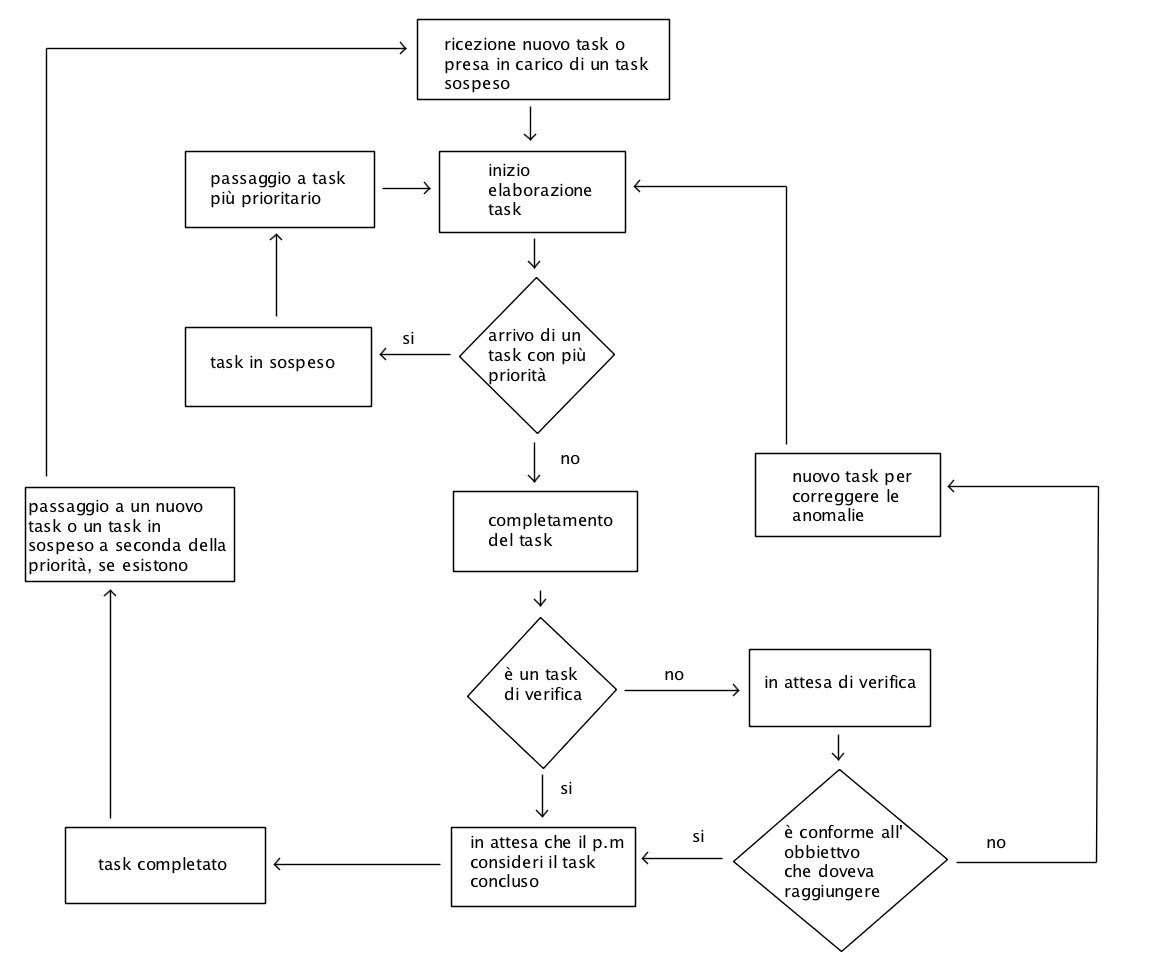
\includegraphics[scale=0.8]{lavorazione_task.jpg}
	\caption{Ciclo di vita di un task}
\end{figure}



\paragraph{Creazione di un task}
Per la creazione di un nuovo singolo \termine{task} bisogna seguire le seguenti
istruzioni:
\begin{enumerate}
  \item Dalla pagina principale di \termine{Wrike} selezionare il progetto interessato (\progetto).
  \item Selezionare la voce \textbf{Nuova attività} e compilare il \termine{task} nel seguente modo:
    \begin{itemize}
      \item \textbf{Nome task:} assegnare un nome identificativo al \termine{task} seguito dalla \termine{milestone} corrispondente (se necessaria).
      \item \textbf{Aggiungi descrizione:} inserire una descrizione breve ma
      concisa del \termine{task}.
      \item \textbf{Allega file:} allegare, eventualmente, file utili alla realizzazione del task.
      \item \textbf{Priorità:} inserire, opzionalmente, una priorità al \termine{task}.
    \end{itemize}
\end{enumerate}


\paragraph{Modifica di un task}
Per modificare un \termine{task} seguire le seguenti istruzioni:
\begin{itemize}
  \item Selezionare il \termine{task} da modificare.
  \item Dalla pagina proposta selezionare il campo che si vuole modificare.
  \item Completata la modifica premere il pulsante \textbf{Invio}.
\end{itemize}

\paragraph{Completamento di un task}
Dopo che il verificatore avrà appurato che il \termine{task} soddisfa i requisiti richiesti, e quindi è stato completato secondo le \NdP, potrà procedere con il suo completamento ottenibile tramite le seguenti operazioni:
\begin{itemize}
  \item Selezionare il \termine{task} da segnare come completato.
  \item Cliccare nella checkbox apposita segnando il termine come \textbf{"Completato"}.
\end{itemize}
Il lavoro viene quindi considerato concluso da questo momento, ma potrebbe essere riportato nello stato \textbf{"In corso"} nel caso in cui:
\begin{itemize}
  \item Il \Pm\ non approvi il documento.
  \item Il \Ver\, dopo un secondo controllo sui \termine{task} a lui assegnati, si accorga di errori e/o incompletezze. 
\end{itemize}

\subsection{Processo di Formazione}
\subsubsection{Descrizione}
Il processo di formazione consiste nel fornire e mantenere tutti i membri del gruppo preparati e in grado di lavorare efficacemente ed efficientemente nella produzione e nella gestione del software.

\subsubsection{Implementazione}
Il \termine{team} ha deciso che la formazione dei membri del gruppo non sarà di pertinenza del gruppo stesso, bensì un dovere del singolo che dovrà intraprendere azioni di autoapprendimento nel caso le sue conoscenze fossero insufficienti al completamento del suo lavoro.

\subsubsection{Materiale di Formazione}
Essendo il processo di formazione riguardante il singolo, ogni membro del \termine{team} che raccolga materiale interessante lo distribuirà all'interno del gruppo. In questo modo il ripresentarsi di problemi di natura similare avrà già parte della soluzione trovata. Eventualmente un membro del \termine{team} può anche chiedere delucidazioni alla persone che in precedenza aveva già trovato una soluzione al medesimo problema.


%
% la parte riguardante la lista di controllo è stata eliminata in quanto
% il prof. stesso ha detto che l improvement dei processi è un processo lungo
% che non riguarda un progetto della durata simile alla nostro
%
%
%\subsection{Lista di controllo}
%Durante l'applicazione della tecnica del \textit{Walkthrough\ped{G}} ai documenti sono stati riportati
%più frequentemente i seguenti errori:
%\begin{itemize}
 % \item\textbf{Norme stilistiche}:
  %\begin{itemize}
   % \item La prima parola di una voce dell'elenco puntato non inizia con una lettera maiuscola.
%    \item La voce dell'elenco puntato termina con un punto anziché con un punto e virgola o viceversa.
 %   \item I due punti in grassetto.
  %  \item Errori di battitura.
    
  %\end{itemize}

  %\item\textbf{Italiano}:
  %\begin{itemize}
   % \item Maiuscole usate impropriamente.
    
  %\end{itemize}

  %\item\textbf{\LaTeX}:
  %\begin{itemize}
  %\item Mancato utilizzo dei comandi \LaTeX{} personalizzati.

  %\end{itemize}
  
  %\item\textbf{Casi d'Uso}:
  %\begin{itemize}
%\item Mancato rispetto del template stabilito per i punti trattati nei casi d'uso.
 % \end{itemize}

	%\item\textbf{Glossario}:
	%\begin{itemize}
	%	\item Sono stati evidenziati dei termini che non andavano nel \textit{\glossario{}}.
	%	\item Non sono stati evidenziati dei termini che sono presenti nel \textit{\glossario{}}.
	%\end{itemize}

%\end{itemize}


\end{document}
